%!TEX program = xelatex
% 完整编译: xelatex -> biber/bibtex -> xelatex -> xelatex
\documentclass[12pt,a4paper,citestyle=gb7714-2015, bibstyle=gb7714-2015,bibtex]{HDUPaper}

\begin{document}
\thispagestyle{empty}
\grade{(2021级)}% 年级
\title{基于单片机的振动测量仪设计}% 论文题目
\school{理学院}% 所在学院
\major{光电信息科学与工程}% 所在专业
\id{21xxxxxx}% 学号
\name{Axia}% 姓名
\teacher{Axia's Teacher}% 导师
\fancyhc{杭州电子科技大学单片机课程设计}% 页眉中
\maketitle
\begin{center}
\section*{\heiti\Large 摘~~~要}
\end{center}
\vspace{1em}

这是摘要这是摘要这是摘要这是摘要这是摘要这是摘要这是摘要这是摘要这是摘要这是摘要.
\subsubsection*{联系作者}
(暂时不想在\faGithub 上透露其他联系方式...)

  \faEnvelope\ \email{xiamyphys@gmail.com}

\keywords{关键词,关键词,关键词,}
\newpage\thispagestyle{empty}
\begin{center}
\section*{\heiti\Large ABSTRACT}
\end{center}

This abstract This abstract This abstract This abstract This abstract This abstract This abstract This abstract This abstract This abstract 

\textbf{Keywords: }Keywords, Keywords, Keywords, 
\newpage\thispagestyle{empty}
\begin{center}
  \tableofcontents
\end{center}
\newpage
\myemptypage
\setcounter{page}{1}
\begin{center}
\section{引言}
\end{center}

\subsection{引言子}
单片机是一块用于对系统或设备进行控制的集成电路芯片,相当于一个微型计算机系统,上面集成了微处理器、存储器及各种输入/输出接口,其中包括CPU、SRAM、FLASH、IO口和中断系统、定时器/计数器等.单片机始于上世纪70年代,随着单片机技术的发展,单片机中可以兼容不同厂商的不同操作系统,可以实现跨平台、跨系统正常运行,一些比较高级的单片机能够兼容Windows和Linux操作系统\cite{cn5}.
\subsubsection*{单片机特点}
其结构非常简单,方便用户进行操作,采用模块化进行设计.单片机具有很高的稳定性,能够长时间保持无故障状态,具有很强的处理能力,能够快速的进行反应.在工作状态下运行的电压很低,消耗的功率很小,方便用户进行携带.具备很强的控制功,在不同的环境中能够正常运行.单片机将程序存储器和数据存储器进行严格分开,I/O引脚具备很好的扩展能力,单片机的体积非常小生产成本非常低可以实现批量化生产,能够组成各种智能化的设备控制系统.单片机能够在各种干扰信息的环境中正常运行,能够在各种环境差的情况中稳定运行,具备其他系统无法比拟的优势.
\subsubsection*{控制原理}
通过控制单片机的40个引脚输出的高低电平进行控制,最后达到控制内外资源的运行目的,因为内部为一些晶体管,可以通过控制晶体管的导通状态而组成不同的逻辑电路,达到不同功能.数字电路中单片机只有高和低两种电平.如若定义单片机为TTL电平则为高电平为$+5\mathrm{V}$、低电平为$0\mathrm{V}$;若定义单片机为计算机串口RS-232的电平则高电平为$+12\mathrm{V}$低电平为$-12\mathrm{V}$.所以单片机与计算机之间进行通讯时需要加电平转换芯片max232.
\subsubsection*{应用范围}
\begin{enumerate}
  \item 军事方面:利用单片机对导弹的导航装置进行设计
  \item 飞机设计:利用单片机对飞机的各种显示仪表进行设计
  \item 计算机设计:利用单片机实现对设备的实时控制和数据处理
  \item 嵌入式领域:工业机器人、智能化仪器设备、IC卡、安全保障系统等
\end{enumerate}
\subsection{振动测量系统概述}
振动测量仪是一款对机器运行状态进行监测的仪器,具有振动检测、轴承状态分析和红外线温度测量等功能.这款仪器操作起来非常简单,当设备存在故障时,仪器能够自动提示报警,能够对机械运行状态进行实时监测,及时发现机械故障问题,保证设备能够正常、可靠运行.振动测量仪可以对机械设备振动速度、加速度和位移值等指标进行测量\cite{cn1,en1}.仪器能够自动对机械设备运行状态中的振动速度读数与其内置的振动标准进行比较,当读值超出标准时,自动指示机器报警状态.振动测量仪被广泛的应用于不同的行业,可以对重要建筑物和桥梁进行常规检查,能够用于突发的地震监测,获得物体的振动量大小.如果将振动检测仪和加速度传感器进行集成,整合成为多功能仪器,能够准确采集到物理运动产生的位移、速度等指标数据.

\subsection{课程设计任务和要求}
\begin{enumerate}
  \item 了解振动测量仪的原理
  \item 根据振动测量仪的原理,设计出其硬件模块和软件程序框图
\end{enumerate}
\newpage
\begin{center}
  \section{振动测量的原理}
\end{center}
\subsection{振动的基本理论}
振动分为正弦振动和随机振动两种,生活中更常见的是随机振动.以下两图分别展现了正弦和随机振动的时域描述.图\ref{fig:2-1}和图\ref{fig:2-2}分别展现了正弦和随机振动的时域描述\cite{en2}.
\begin{figure}[h]
  \centering
  \begin{minipage}[t]{0.48\textwidth}
  \centering
  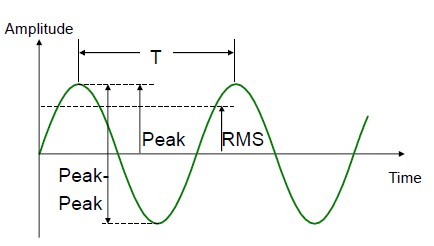
\includegraphics[width=0.93\textwidth]{image/1.jpg}
  \caption{正弦振动时域图}\label{fig:2-1}
  \end{minipage}
  \begin{minipage}[t]{0.48\textwidth}
  \centering
  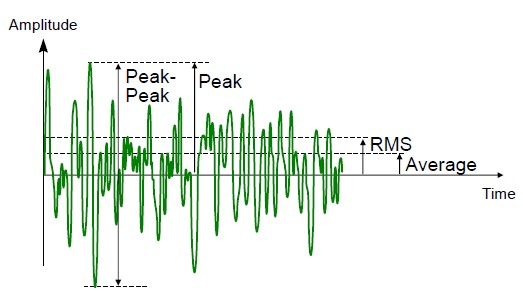
\includegraphics[width=0.93\textwidth]{image/2.jpg}
  \caption{随机振动时域图}\label{fig:2-2}
  \end{minipage}
  \end{figure}

\subsection{振动测量仪原理}
\subsubsection{振动测量仪的测量内容}
对振动物体上某个点的位置移动、速度、加速度和相位等参数的测量,了解被测对象的振动状态,对测试对象的振动量级进行评定,实现对设备的实时监测、故障诊断和性能评估;其次可以进行结构或部件的动态特性测量,将一种振动力施加到被测部件上,使部件进行振动,对部件的振动参数和动态性能进行测量,这些参数包括阻尼、阻抗、频率、模态等,通过测试的内容不同可以将测试分为振动环境模拟试验、机械阻抗试验和频率响应试验等.
\subsubsection{振动测量仪的数据采集过程}
\begin{enumerate}
  \item 向计算机控制仪软件输入模拟振动试验的图谱要求,点击启动按钮,则驱动输出一定幅值的控制信号给功率放大器,经过功率放大器把信号放大后输出给振动台内、外驱动线圈,由于振动台中的励磁线圈接通励磁电源后,在台体构成的磁回路的环形工作气隙中会形成径向直流磁场,而感应环正好位于这个充满直流磁场的工作气隙的中间,所以当感应环中通过驱动线圈中的交变电流的感应产生的感应电流产生后,与稳定的直流磁场相互作用而产生点动力来带动动圈沿轴向方向即推力方向运动,其推力公式\cite{en3}为
  $$F=BIL\eqno(2.1)$$
  其中,$F$为振动时的推力大小,$B$为工作气隙中的磁感应强度,$I$为驱动线圈电流,$L$为驱动线圈导线的有效长度.
  \item 通过粘接或螺接在试件上面的加速度传感器,把测量的振动信号变换成电荷信号(或者直接变换成电压信号输出给控制仪)输出给电荷放大器,经过电荷放大器变换成电压信号后输出给控制仪,控制仪通过这个回馈信号来调整输出给功率放大器的控制信号,从而实现振动试验系统的闭环控制.而振动测量仪采集信号恰恰可以在振动台上再粘贴一个传感器,将振动台产生的振动值测量出来,可以相互的对比验证.如图\ref{fig:2-3}所示.
  \begin{figure}[h]
    \centering % 图片居中
    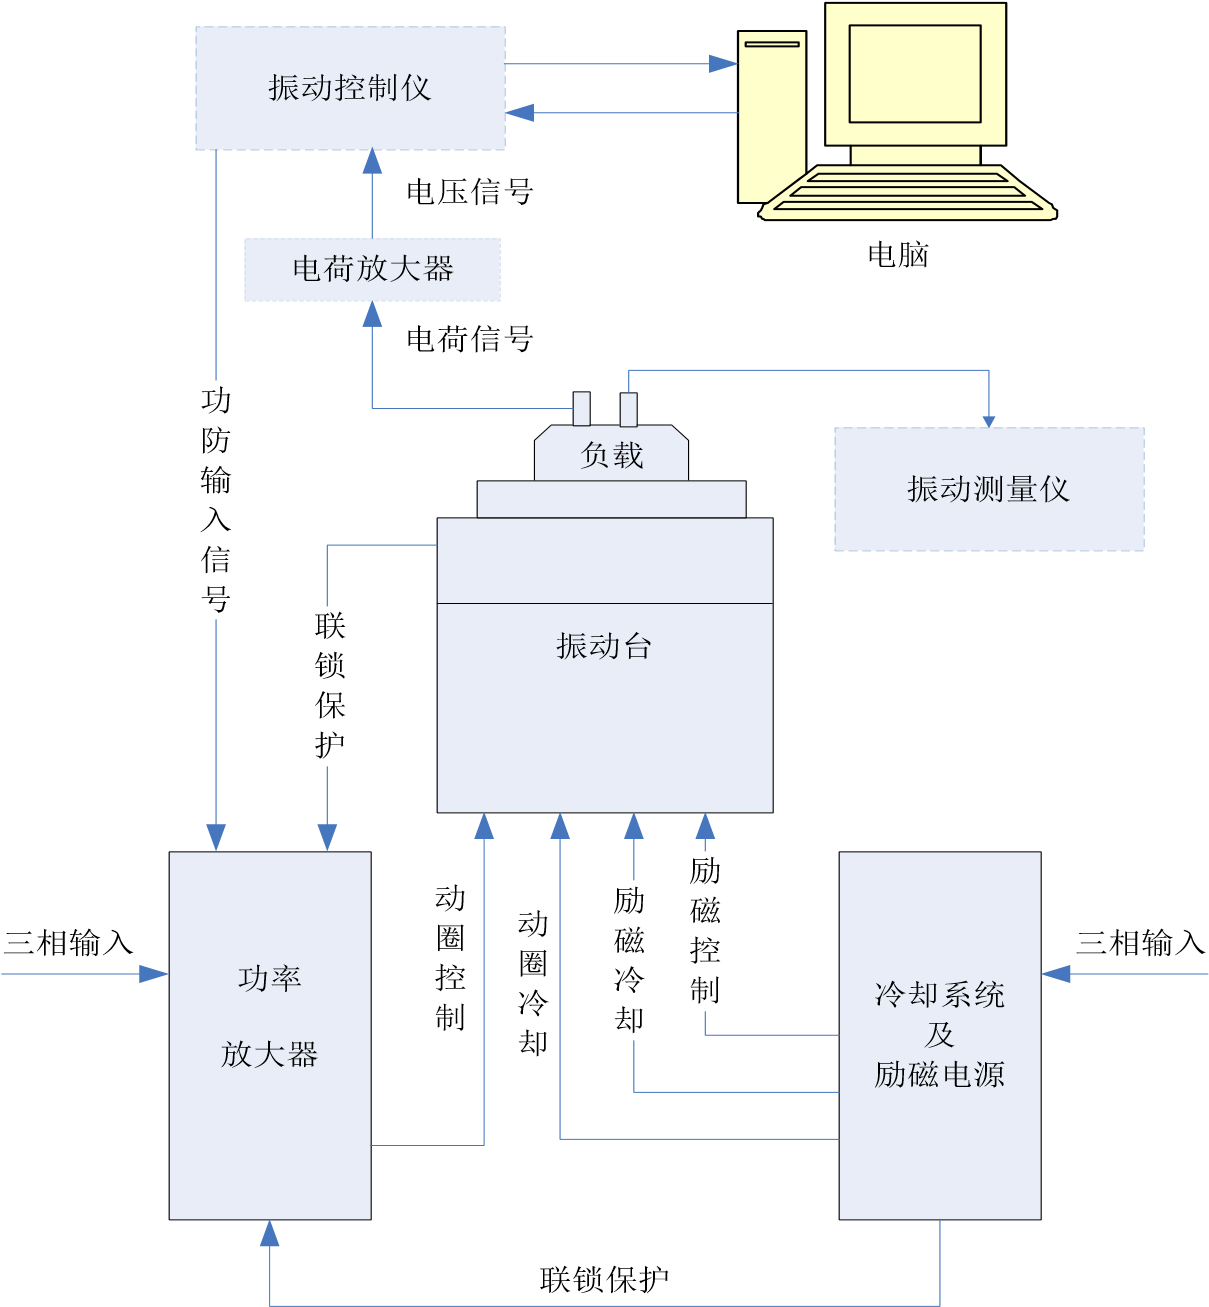
\includegraphics[width=0.93\textwidth]{image/3.png}
    \caption{振动台工作原理及测量仪采集示意图}
    \label{fig:2-3}
  \end{figure}
\end{enumerate}
\newpage

\printbibliography[heading=bibintoc, title=\ebibname]% 输出参考文献
\end{document}
